\chapter{Implementation} % (fold)
\label{chap:Implementation}
% python protocol "Next Header:8,Hdr Ext Len:8,Routing Type:8,Num. Dst:8,Flags:2,Hops:6,Reserved:24,Delivery Map:32,Router Map:32,Address List:128"
% python protocol "Next Header:8,Hdr Ext Len:8,Routing Type:8,Segments Left:8,Num. Dst:8,Flags:2,Hops:6,Reserved:16,Delivery Map:32,Router Map:32,Address List:128"

\begin{figure}[h!]
\centering
\begin{lstlisting}[xleftmargin=.07\textwidth]
 0                   1                   2                   3
 0 1 2 3 4 5 6 7 8 9 0 1 2 3 4 5 6 7 8 9 0 1 2 3 4 5 6 7 8 9 0 1
+-+-+-+-+-+-+-+-+-+-+-+-+-+-+-+-+-+-+-+-+-+-+-+-+-+-+-+-+-+-+-+-+
|  Next Header  |  Hdr Ext Len  |  Routing Type |    Num. Dst   |
+-+-+-+-+-+-+-+-+-+-+-+-+-+-+-+-+-+-+-+-+-+-+-+-+-+-+-+-+-+-+-+-+
|Fl.|    Hops   |                    Reserved                   |
+-+-+-+-+-+-+-+-+-+-+-+-+-+-+-+-+-+-+-+-+-+-+-+-+-+-+-+-+-+-+-+-+
|                          Delivery Map                         |
+-+-+-+-+-+-+-+-+-+-+-+-+-+-+-+-+-+-+-+-+-+-+-+-+-+-+-+-+-+-+-+-+
|                           Router Map                          |
+-+-+-+-+-+-+-+-+-+-+-+-+-+-+-+-+-+-+-+-+-+-+-+-+-+-+-+-+-+-+-+-+
|                                                               |
.                                                               .
.                          Address List                         .
.                                                               .
|                                                               |
+-+-+-+-+-+-+-+-+-+-+-+-+-+-+-+-+-+-+-+-+-+-+-+-+-+-+-+-+-+-+-+-+
\end{lstlisting}
\caption{Python: MEADcast Header}
\end{figure}

\begin{figure}[h!]
\centering
\begin{lstlisting}[xleftmargin=.07\textwidth]
 0                   1                   2                   3
 0 1 2 3 4 5 6 7 8 9 0 1 2 3 4 5 6 7 8 9 0 1 2 3 4 5 6 7 8 9 0 1
+-+-+-+-+-+-+-+-+-+-+-+-+-+-+-+-+-+-+-+-+-+-+-+-+-+-+-+-+-+-+-+-+
|  Next Header  |  Hdr Ext Len  |  Routing Type | Segments Left |
+-+-+-+-+-+-+-+-+-+-+-+-+-+-+-+-+-+-+-+-+-+-+-+-+-+-+-+-+-+-+-+-+
|    Num. Dst   |Fl.|    Hops   |            Reserved           |
+-+-+-+-+-+-+-+-+-+-+-+-+-+-+-+-+-+-+-+-+-+-+-+-+-+-+-+-+-+-+-+-+
|                          Delivery Map                         |
+-+-+-+-+-+-+-+-+-+-+-+-+-+-+-+-+-+-+-+-+-+-+-+-+-+-+-+-+-+-+-+-+
|                           Router Map                          |
+-+-+-+-+-+-+-+-+-+-+-+-+-+-+-+-+-+-+-+-+-+-+-+-+-+-+-+-+-+-+-+-+
|                                                               |
.                                                               .
.                          Address List                         .
.                                                               .
|                                                               |
+-+-+-+-+-+-+-+-+-+-+-+-+-+-+-+-+-+-+-+-+-+-+-+-+-+-+-+-+-+-+-+-+

\end{lstlisting}
\caption{Current: MEADcast Header}
\end{figure}

% \paragraph{Routing Type} % (fold)
% \label{par:Routing Type}
% Since there is no existing Routing Type for MEADcast we use the experimental
%     values of 253 and 254 according to RFC3692 \cite{rfc3692_ipv6_rt_type}.
% % paragraph Routing Type (end)
%
% \paragraph{Segments Left} % (fold)
% \label{par:Segments Left}
% Fixed to zero and is not altered by MEADcast routers.
% Thereby intermediate nodes, which does not recognize the used Routing type
%     value must ignore the MEADcast header and process the next header
%     \cite{rfc8200_ipv6_hdr}.
% % paragraph Segments Left (end)
%
% \paragraph{Number of Destinations} % (fold)
% \label{par:Number of Destinations}
% Indicates the length of the address list.
% % paragraph Number of Destinations (end)
%
% \paragraph{Flags} % (fold)
% \label{par:Flags}
% 1 bit discovery and 1 bit response.
% % paragraph Flags (end)
%
% \paragraph{Hops} % (fold)
% \label{par:Hops}
% This field is used during the discovery phase.
% The sender initializes the field with zero and gets incremented by each
%     MEADcast router.
% % paragraph Hops (end)
%
% \paragraph{Delivery Map} % (fold)
% \label{par:Delivery Map}
% Bitmap indicating, whether an address in the address list needs to be
%     delivered.
% % paragraph Delivery Map (end)
%
% \paragraph{Router Map} % (fold)
% \label{par:Router Map}
% Immutable bitmap indicating, whether an address in the address list is a router.
% % paragraph Router Map (end)
%
% \paragraph{Address List} % (fold)
% \label{par:Address List}
% List of length ``\texttt{Number of Destinations}'' containing IPv6 addresses.
% % paragraph Address List (end)

\bgroup
\begin{table}[h!]
\centering
\def\arraystretch{1.5}%  1 is the default
\setlength{\tabcolsep}{1.2em}
\begin{tabularx}{\textwidth}{lX}
% \toprule
% \textbf{Field}& \textbf{Desciption} \\
% \midrule
Routing Type  & Since there is no existing Routing Type for MEADcast we use the
                experimental values of 253 and 254 according to RFC3692
                \cite{rfc3692_ipv6_rt_type}.\\
Segments Left & Fixed to zero and is not altered by MEADcast routers. Thereby
                intermediate nodes, which does not recognize the used Routing
                type value must ignore the MEADcast header and process the next
                header \cite{rfc8200_ipv6_hdr}.\\
Num. Dst.     & Indicates the length of the address list. \\
Flags         & 1 bit discovery, 1 bit response        \\
Hops          & This field is used during the discovery phase. The sender
                initializes the field with zero and gets incremented by each
                MEADcast router. \\
Delivery Map  & Bitmap indicating, whether an address in the address list needs
                to be delivered.\\
Router Map    & Bitmap indicating, whether an address in the address list is a
                router.\\
Address List  & Variable length list of IPv6 addresses. \\
% \bottomrule
\end{tabularx}
\caption{MEADcast Header field description}
\label{tab:my-table}
\end{table}
\egroup

\section{Router} % (fold)
\label{sec:Router}

% section Router (end)


\section{Testbed} % (fold)
\label{sec:Testbed_Implementation}
\subsection{Topology} % (fold)
\label{sub:Topology}

\begin{figure}
    \begin{center}
        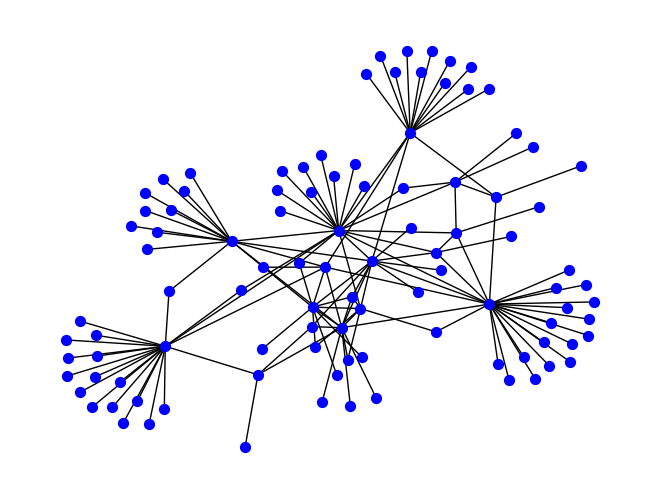
\includegraphics[width=0.95\textwidth]{Bilder/net_topo_as_100.png}
    \end{center}
    \caption{AS 100}
    \label{fig:as100}
\end{figure}

\begin{figure}
    \begin{center}
        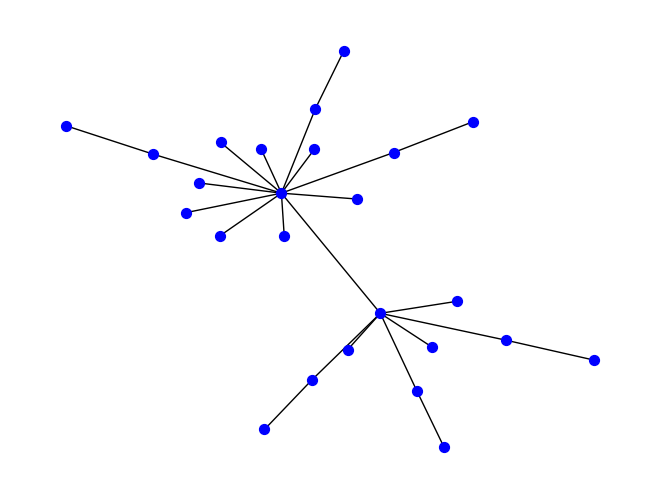
\includegraphics[width=0.7\textwidth]{Bilder/net_topo_ba_25_1.png}
    \end{center}
    \caption{Barabasi Albert 25/1 v1}
    \label{fig:ba_25_1_1}
\end{figure}
\begin{figure}
    \begin{center}
        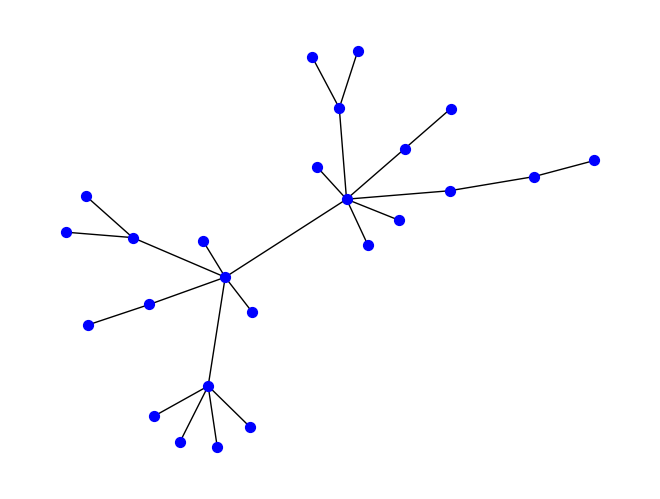
\includegraphics[width=0.7\textwidth]{Bilder/net_topo_ba_25_1_1.png}
    \end{center}
    \caption{Barabasi Albert 25/1 v2}
    \label{fig:ba_25_1_2}
\end{figure}
\begin{figure}
    \begin{center}
        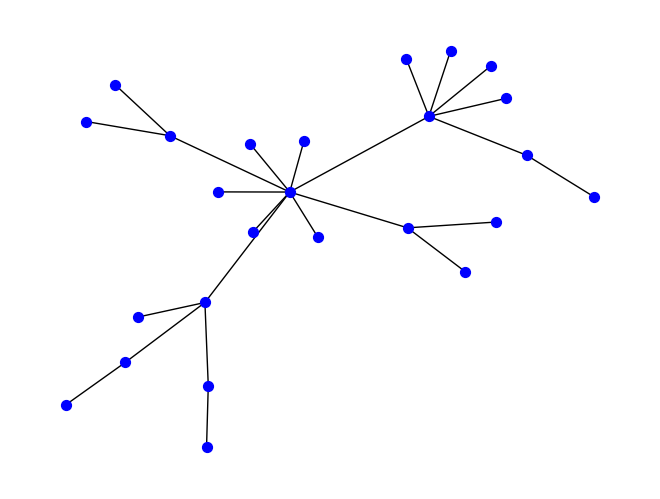
\includegraphics[width=0.7\textwidth]{Bilder/net_topo_ba_25_1_2.png}
    \end{center}
    \caption{Barabasi Albert 25/1 v3}
    \label{fig:ba_25_1_3}
\end{figure}

% subsection Topology (end)
% section Testbed (end)


% chapter Implementation (end)
